\subsection{Allgemeines}
\begin{frame}{Scheduling - Definitionen}
	\uncover<1>{	
	\begin{block}{Scheduling}
		Aufteilung von CPU-Zeit auf um die Ressource konkurrierende Prozesse oder Threads
	\end{block}
	}
	\uncover<2>{
	\begin{block}{Scheduling-Strategie}
		Verfahren nachdem ein Scheduling vorgenommen wird
	\end{block}
	}
	\uncover<3>{
	\begin{block}{Verdrängend und nicht Verdrängend}
		nicht Verdrängend: Sobald ein Prozess die Priorität zugesprochen bekommt, arbeitet er durch \\
		Verdrängend: Sobald ein Prozess nach Strategie höherer Priorität erscheint, wird der arbeitende Prozess ersetzt
	\end{block}
	}
\end{frame}

\begin{frame}{Strategie-Ziele}
	\begin{itemize}
		\item<1-> \textbf{Allgemein}
		\begin{itemize}[<+->]
			\item Ressource optimal ausnutzen (Balance)
			\item Keinen Prozess benachteiligen (Fairness)
		\end{itemize}
		\item<3->\textbf{Stacksysteme}
		\begin{itemize}[<+->]
			\item Maximierung des Durchsatzes %(der geleisteten Arbeit)
			\item Minimierung der Durchlaufzeit
			\item Maximierung der CPU-Auslastung
		\end{itemize}
		\item<6-> \textbf{Interaktive Systeme}
		\begin{itemize}[<+->]
			\item Reduktion der Antwortzeit
			\item Proportionalität gewährleisten %(Benutzererwartung erfüllen)
		\end{itemize}
		\item<8-> \textbf{Echtzeitsysteme}
		\begin{itemize}[<+->]
			\item Deadlines einhalten
			\item Vorhersagbarkeit %(Reduktion des Qualitätsverlustes in Multimedia-Systemen)
		\end{itemize}
	\end{itemize}
\end{frame}

\begin{frame}{Beispiel: Round Robin}
	\begin{tabular}{l||c|c|c|c}
		Auftrag               & \(A_1\)  & \(A_2\)  & \(A_3\) & \(A_4\) \\ \hline \hline
		Ankunftszeit		  & 0        &  4		& 5       & 8       \\ \hline
		Bedienzeitanforderung & 6        &  4       & 2       & 6       \\
	\end{tabular}\quad \\ \quad \\
	Zeitscheibengröße: \(\Delta t = 2\) \\
	Queue\(_{t0}\):[\(A_1\)] \\
	Queue\(_{t2}\):[] \\
	\begin{center}
	\begin{blockgraph}{25}{1}{0.4}
	    \bglabelxx{0}
	    \bglabelxx{5}
	    \bglabelxx{10}
	    \bglabelxx{15}
	    \bglabelxx{20}
   	 	\bglabelxx{25}
    \end{blockgraph}
	\end{center}
\end{frame}

\begin{frame}{Beispiel: Round Robin}
	\begin{tabular}{l||c|c|c|c}
		Auftrag               & \(A_1\)  & \(A_2\)  & \(A_3\) & \(A_4\) \\ \hline \hline
		Ankunftszeit		  & 1        &  4		& 5       & 8       \\ \hline
		Bedienzeitanforderung & 6        &  4       & 2       & 6       \\
	\end{tabular}\quad \\ \quad \\
	Zeitscheibengröße: \(\Delta t = 2\) \\
	Queue\(_{t4}\):[\(A_2\)] \\
	\quad \\
	\begin{center}
	\begin{blockgraph}{25}{1}{0.4}
	    \bglabelxx{0}
	    \bglabelxx{5}
	    \bglabelxx{10}
	    \bglabelxx{15}
	    \bglabelxx{20}
   	 	\bglabelxx{25}
    
    	\bgblock{0}{2}{$A_1$}
    	\bgblock{2}{4}{$A_1$}
    	\bgemptyblock{4}{5}
    \end{blockgraph}
	\end{center}
\end{frame}

\begin{frame}{Beispiel: Round Robin}
	\begin{tabular}{l||c|c|c|c}
		Auftrag               & \(A_1\)  & \(A_2\)  & \(A_3\) & \(A_4\) \\ \hline \hline
		Ankunftszeit		  & 1        &  4		& 5       & 8       \\ \hline
		Bedienzeitanforderung & 6        &  4       & 2       & 6       \\
	\end{tabular}\quad \\ \quad \\
	Zeitscheibengröße: \(\Delta t = 2\) \\
	Queue\(_{t7}\):[\(A_1, A_3\)] \\
	\quad \\
	\begin{center}
	\begin{blockgraph}{25}{1}{0.4}
	    \bglabelxx{0}
	    \bglabelxx{5}
	    \bglabelxx{10}
	    \bglabelxx{15}
	    \bglabelxx{20}
   	 	\bglabelxx{25}
    
    	\bgblock{0}{2}{$A_1$}
    	\bgblock{2}{4}{$A_1$}
    	\bgemptyblock{4}{5}
    	\bgblock{5}{7}{$A_2$}
    	\bgemptyblock{7}{8}
    \end{blockgraph}
	\end{center}
\end{frame}

\begin{frame}{Beispiel: Round Robin}
	\begin{tabular}{l||c|c|c|c}
		Auftrag               & \(A_1\)  & \(A_2\)  & \(A_3\) & \(A_4\) \\ \hline \hline
		Ankunftszeit		  & 1        &  4		& 5       & 8       \\ \hline
		Bedienzeitanforderung & 6        &  4       & 2       & 6       \\
	\end{tabular}\quad \\ \quad \\
	Zeitscheibengröße: \(\Delta t = 2\) \\
	Queue\(_{t10}\):[\(A_3, A_2,A_4\)] \\
	\quad \\
	\begin{center}
	\begin{blockgraph}{25}{1}{0.4}
	    \bglabelxx{0}
	    \bglabelxx{5}
	    \bglabelxx{10}
	    \bglabelxx{15}
	    \bglabelxx{20}
   	 	\bglabelxx{25}
    
    	\bgblock{0}{2}{$A_1$}
    	\bgblock{2}{4}{$A_1$}
    	\bgemptyblock{4}{5}
    	\bgblock{5}{7}{$A_2$}
    	\bgemptyblock{7}{8}
    	\bgblock{8}{10}{$A_1$}
    	\bgemptyblock{10}{11}
    \end{blockgraph}
	\end{center}
\end{frame}

\begin{frame}{Beispiel: Round Robin}
	\begin{tabular}{l||c|c|c|c}
		Auftrag               & \(A_1\)  & \(A_2\)  & \(A_3\) & \(A_4\) \\ \hline \hline
		Ankunftszeit		  & 1        &  4		& 5       & 8       \\ \hline
		Bedienzeitanforderung & 6        &  4       & 2       & 6       \\
	\end{tabular}\quad \\ \quad \\
	Zeitscheibengröße: \(\Delta t = 2\) \\
	Queue\(_{t13}\):[\(A_2,A_4\)] \\
	\quad \\
	\begin{center}
	\begin{blockgraph}{25}{1}{0.4}
	    \bglabelxx{0}
	    \bglabelxx{5}
	    \bglabelxx{10}
	    \bglabelxx{15}
	    \bglabelxx{20}
   	 	\bglabelxx{25}
    
    	\bgblock{0}{2}{$A_1$}
    	\bgblock{2}{4}{$A_1$}
    	\bgemptyblock{4}{5}
    	\bgblock{5}{7}{$A_2$}
    	\bgemptyblock{7}{8}
    	\bgblock{8}{10}{$A_1$}
    	\bgemptyblock{10}{11}
    	\bgblock{11}{13}{$A_3$}
    	\bgemptyblock{13}{14}
    \end{blockgraph}
	\end{center}
\end{frame}

\begin{frame}{Beispiel: Round Robin}
	\begin{tabular}{l||c|c|c|c}
		Auftrag               & \(A_1\)  & \(A_2\)  & \(A_3\) & \(A_4\) \\ \hline \hline
		Ankunftszeit		  & 1        &  4		& 5       & 8       \\ \hline
		Bedienzeitanforderung & 6        &  4       & 2       & 6       \\
	\end{tabular}\quad \\ \quad \\
	Zeitscheibengröße: \(\Delta t = 2\) \\
	Queue\(_{t16}\):[\(A_4\)] \\
	\quad \\
	\begin{center}
	\begin{blockgraph}{25}{1}{0.4}
	    \bglabelxx{0}
	    \bglabelxx{5}
	    \bglabelxx{10}
	    \bglabelxx{15}
	    \bglabelxx{20}
   	 	\bglabelxx{25}
    
    	\bgblock{0}{2}{$A_1$}
    	\bgblock{2}{4}{$A_1$}
    	\bgemptyblock{4}{5}
    	\bgblock{5}{7}{$A_2$}
    	\bgemptyblock{7}{8}
    	\bgblock{8}{10}{$A_1$}
    	\bgemptyblock{10}{11}
    	\bgblock{11}{13}{$A_3$}
    	\bgemptyblock{13}{14}
    	\bgblock{14}{16}{$A_2$}
    	\bgemptyblock{16}{17}
    \end{blockgraph}
	\end{center}
\end{frame}

\begin{frame}{Beispiel: Round Robin}
	\begin{tabular}{l||c|c|c|c}
		Auftrag               & \(A_1\)  & \(A_2\)  & \(A_3\) & \(A_4\) \\ \hline \hline
		Ankunftszeit		  & 1        &  4		& 5       & 8       \\ \hline
		Bedienzeitanforderung & 6        &  4       & 2       & 6       \\
	\end{tabular}\quad \\ \quad \\
	Zeitscheibengröße: \(\Delta t = 2\) \\
	Queue\(_{t19}\):[\(\)] \\
	Queue\(_{t21}\):[\(\)] \\
	\begin{center}
	\begin{blockgraph}{25}{1}{0.4}
	    \bglabelxx{0}
	    \bglabelxx{5}
	    \bglabelxx{10}
	    \bglabelxx{15}
	    \bglabelxx{20}
   	 	\bglabelxx{25}
    
    	\bgblock{0}{2}{$A_1$}
    	\bgblock{2}{4}{$A_1$}
    	\bgemptyblock{4}{5}
    	\bgblock{5}{7}{$A_2$}
    	\bgemptyblock{7}{8}
    	\bgblock{8}{10}{$A_1$}
    	\bgemptyblock{10}{11}
    	\bgblock{11}{13}{$A_3$}
    	\bgemptyblock{13}{14}
    	\bgblock{14}{16}{$A_2$}
    	\bgemptyblock{16}{17}
    	\bgblock{17}{19}{$A_4$}
    	\bgblock{19}{21}{$A_4$}
    	\bgblock{21}{23}{$A_4$}
    \end{blockgraph}
	\end{center}
\end{frame}

\subsection{Strategien, interaktive und Stacksysteme}
\begin{frame}{First In, First Out}
	\begin{itemize}
		\item nicht verdrängend \(\Rightarrow\) geringste Kosten für Prozesswechsel
		\item einfach vorstellbare Strategie
		\item Erster rechenbereiter Prozess bekommt als erster Rechenzeit, zweiter als zweites
		\item durch Queues schnell implementierbar
	\end{itemize}
\end{frame}

\begin{frame}{Shortest Job First}
	\begin{itemize}
		\item nicht verdrängende Strategie
		\item mengenbasiert, Prozess mit geringsten Anforderungen bekommt höchste Priorität
		\item Durchsatz nachweislich optimal
		\item nicht Fair (potentiell ''verhungernde'' Prozess)
	\end{itemize}
\end{frame}

\begin{frame}{Shortest Remaining Time Next}
	\begin{itemize}
		\item verdrängende Variante von Shortest Job First
		\item berücksichtigt wird die verbleibende Anforderung
		\item Fairnessprobleme bleiben
	\end{itemize}
\end{frame}

\begin{frame}{Round Robin}
	\begin{itemize}
		\item<2-> verdrängende Strategie
		\item<3-> CPU-Zeit in Zeitscheiben unterteilt
		\item<4-> Queue-basiert
		\item<5-> implizite Annahme: alle Prozesse gleich wichtig
	\end{itemize}
\end{frame}

\begin{frame}{Priorisiertes Scheduling}
	\begin{itemize}
		\item verdrängende Strategien
		\item Sammelbezeichnung für bestimmte Strategien
		\item Idee: Jeder rechenbereite Prozess bekommt eine Prioritätswertung
		\item Für Interaktivität: dynamisches Anpassen der Priorität 
	\end{itemize}
\end{frame}

\begin{frame}{Prioritätsklassen}
	\begin{itemize}
		\item Prioritäten errechnen teuer
		\item Zusammenfassen von Prozessen zu Klassen
		\item innerhalb der Klassen Round Robin
		\item Anpassen der Prioritäten, verhindert ''verhungern'' der unteren Klassen
	\end{itemize}
\end{frame}

\begin{frame}{Shortest Process Next}
	\begin{itemize}
		\item Shortest Job First für interaktive Systeme
		\item Laufzeitinformationen heuristisch ermittelt
		\item[\(\Rightarrow\)] Profiler benötigt
	\end{itemize}
\end{frame}

\begin{frame}{Fair Share Scheduling}
	\begin{itemize}
		\item Betrachtet Nutzerzugehörigkeit
		\item Stellt Nutzerfairness, nicht Prozessfairness her
	\end{itemize}
\end{frame}

\subsection{Echtzeitsysteme}
\begin{frame}{Periodizität}
	Aufgaben spawnen innerhalb bestimmter Zeitabschnitte (Periode, \(P_i\)) immer wieder. \\
	\begin{center}
		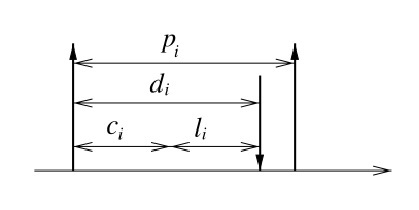
\includegraphics[scale=0.75]{images/periodic}\cite{ESDes}
	\end{center}
\end{frame}

\begin{frame}{Deadlines}
	\uncover<1->{
	\begin{block}{Hard}
		Harte Deadlineverletzung: Es droht eine Katastrophe, ausgelöst durch Systemabsturz. \\
		\(\Rightarrow\) Verletzung nicht tolerabel.
	\end{block}
	}
	\uncover<2->{
	\begin{block}{Soft}
		Weiche Deadlineverletzung: Seltene Fehler verzeihlich. \\
		\(\Rightarrow\) Verletzung ist tolerable, sollte aber trotzdem vermieden werden.
	\end{block}
	}
\end{frame}

\begin{frame}{Schedularisierbarkeit}
	\begin{itemize}
		\item Annahme: optimaler Scheduler
		\item \(C_i\): Zeitanforderung von Task \(i\)
		\item \(P_i\): Periodenlänge von Task \(i\)
	\end{itemize}
	\begin{center}
	\uncover<2>{
		\[\sum\limits_{i=1}^{n}\frac{C_i}{P_i} \leq 1\]
	}
	\end{center}
\end{frame}

\begin{frame}{Schedularisierbarkeit}
	\textbf{Annahmen:}	
	\begin{itemize}
		\item Unendlicher Zeitraum
		\item verschiedene, periodische Tasks
		\item (implizit) Periodenlänge = Deadline
	\end{itemize}
\end{frame}

\begin{frame}{Schedularisierbarkeit}
	\uncover<1->{
	\textbf{Schritt 1:} \\
	Unterteilung der Unendlichkeit in einzelne, den Periodenlängen angepasste Zeitschritte \(\Rightarrow\   	
	Ch = kgv(P_i)\) \\
	}
	\uncover<2->{
	\textbf{Schritt 2:} \\
	Berechnung von \(a(i) = C_i \cdot \frac{Ch}{P_i}\) für alle Aufgaben \\
	}
	\uncover<3->{
	\textbf{Schritt 3:} \\
	Überprüfen: \(\sum\limits_{i=1}^{n}a(i) \leq Ch |n = \text{Anzahl der Prozesse}\) \\
	}
	\uncover<4->{
	\textbf{Schritt 4 (Überführung):} \\
	\(
	\begin{array}{llcl}
		&\sum\limits_{i=1}^{n}a(i) \leq Ch &\Leftrightarrow & 
		\sum\limits_{i=1}^{n}\frac{a(i)}{Ch} \leq 1 \\
		\Leftrightarrow & \sum\limits_{i=1}^{n}\frac{C_i \cdot \frac{Ch}{P_i}}{Ch} \leq 1 & \Leftrightarrow & 
		\sum\limits_{i=1}^{n}\frac{C_i}{P_i} \leq 1
	\end{array}
	\)
	}
\end{frame}

\begin{frame}{Prioritätsinversion}
	\begin{itemize}
		\item Geteilte Ressource
		\item führt potentiell zu Problemen (Bsp: \(A\) muss vor Darstellungsende terminieren)
		\item scheinbare Umkehr der Priorität
	\end{itemize}
	\begin{center}
		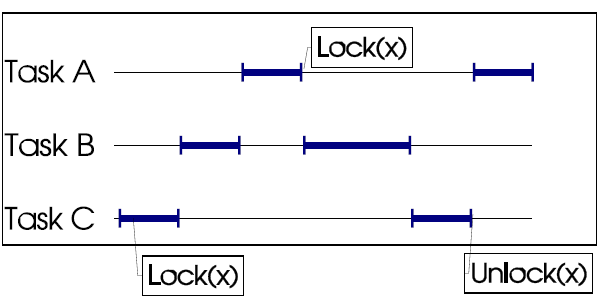
\includegraphics[scale=0.5]{images/prioInv} \cite{jamaicaPic} \\
		\(A > B > C\) wobei \(A\) nach \(B\) nach \(C\) auftritt
	\end{center}
\end{frame}

\begin{frame}{Prioritätsinversion}
	\textbf{Lösung: Prioritätsvererbung}
	\begin{center}
		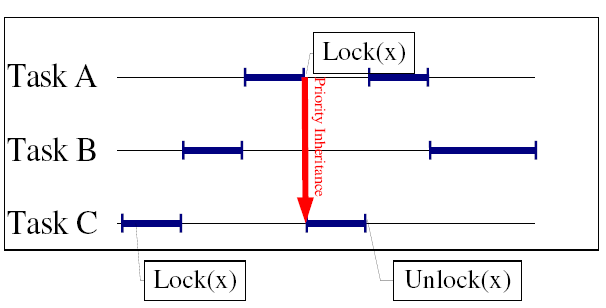
\includegraphics[scale=0.5]{images/prioInh} \cite{jamaicaPic} \\
		\(A > B > C\) wobei \(A\) nach \(B\) nach \(C\) auftritt
	\end{center}
\end{frame}

\begin{frame}{Rate Monotonic Scheduling}
	\begin{itemize}
		\item verdrängende Strategie
		\item statische Prioritäten anhand Periodenlänge
		\item nicht optimal
		\item Schedularisierbarkeit: \(\sum\limits_{i=1}^{n}\frac{C_i}{P_i} \leq n\cdot(2^{\frac{1}{n}}-1)\) \cite{tanenb2009}
		\item nähert sich ln(2) an
	\end{itemize}
\end{frame}

\begin{frame}{RMTS Problembeispiel}
	\begin{center}
	\begin{tabular}{l||c|c|c|c}
		Auftrag               & \(A_1\)  & \(A_2\)  & \(A_3\) & \(A_4\) \\ \hline \hline
		Periodendauer		  & 7        & 11       & 9       & 4       \\ \hline
		Bedienzeitanforderung & 3        &  1       & 2       & 1       \\
	\end{tabular}
	\\ \quad \\ \(\Rightarrow\) Prioritäten: \(A_4 > A_1 > A_3 > A_2\)
	\end{center}
	\begin{center}
	\begin{blockgraph}{25}{1}{0.4}
    	\bglabelxx{0}
    	\bglabelxx{5}
    	\bglabelxx{10}
    	\bglabelxx{15}
    	\bglabelxx{20}
    	\bglabelxx{25}
    
    	\bgblock{0}{1}{$A_4$}
    	\bgblock{1}{4}{$A_1$}
    	\bgblock{4}{5}{$A_4$}
    	\bgblock{5}{7}{$A_3$}
    	\bgblock{7}{8}{$A_1$}
   		\bgblock{8}{9}{$A_4$}
    	\bgblock{9}{11}{$A_4$}
	\end{blockgraph}
	\end{center}
\end{frame}

\begin{frame}{Earliest Deadline First}
	\begin{itemize}
		\item verdrängende Strategie
		\item Prioritätenvergabe anhand der nächsten Deadline
		\item selbe Bedingung, wie optimaler Scheduler
		\item Implementation durch Queue
		\item benötigt nicht zwingend feste Periodenlängen (wie RMTS)
		\item kann mit aperiodischen Tasks umgehen
	\end{itemize}
\end{frame}

\begin{frame}{EDF schaft RMTS-Problem}
	\begin{center}
	\begin{tabular}{l||c|c|c|c}
		Auftrag               & \(A_1\)  & \(A_2\)  & \(A_3\) & \(A_4\) \\ \hline \hline
		Periodendauer		  & 7        & 11       & 9       & 4       \\ \hline
		Bedienzeitanforderung & 3        &  1       & 2       & 1       \\
	\end{tabular}
	\\ \quad \\
	\end{center}
	\begin{center}
	\begin{blockgraph}{25}{1}{0.4}
    	\bglabelxx{0}
    	\bglabelxx{5}
    	\bglabelxx{10}
    	\bglabelxx{15}
    	\bglabelxx{20}
    	\bglabelxx{25}
    	
    	\bgblock{0}{1}{$A_4$}
    	\bgblock{1}{4}{$A_1$}
    	\bgblock{4}{5}{$A_4$}
    	\bgblock{5}{7}{$A_3$}
    	\bgblock{7}{8}{$A_2$}
    	\bgblock{8}{9}{$A_4$}
    	\bgblock{9}{12}{$A_1$}
    	\bgblock{12}{13}{$A_4$}
    	\bgblock{13}{15}{$A_3$}
    	\bgblock{15}{16}{$A_1$}
    	\bgblock{16}{17}{$A_4$}
    	\bgblock{17}{19}{$A_1$}
    	\bgblock{19}{20}{$A_2$}
	    \bgblock{20}{21}{$A_4$}
    	\bgblock{21}{23}{$A_3$}
	\end{blockgraph}
	\end{center}
\end{frame}

\subsection{Preemptive Scheduling}
\begin{frame}{Allgemeines}
	\begin{itemize}
		\item Problem: Tasks voneinander abhängig \(\Rightarrow\) nicht rechenbereit
		\item Was passiert bei Deadlines?
		\item Mit Periodizität der Tasks Schedularisierbarkeit NP-Vollständig \cite{ESDes}
	\end{itemize}
\end{frame}

\begin{frame}{As soon as possible}
	\begin{itemize}
		\item Aufbau des Abhängigkeitsgraphen
		\item Betrachtung der Ursprungsmenge, als berechenbare Elemente
		\item Beliebiges Scheduling der Menge (da voneinander unabhängig)
		\item Neue Elemente nun rechenbereit \(\Rightarrow\) neue Menge
		\item Wiederholung bis alle Knoten besucht
	\end{itemize}
\end{frame}

\begin{frame}{As soon as possible Beispiel}
	\begin{center}
		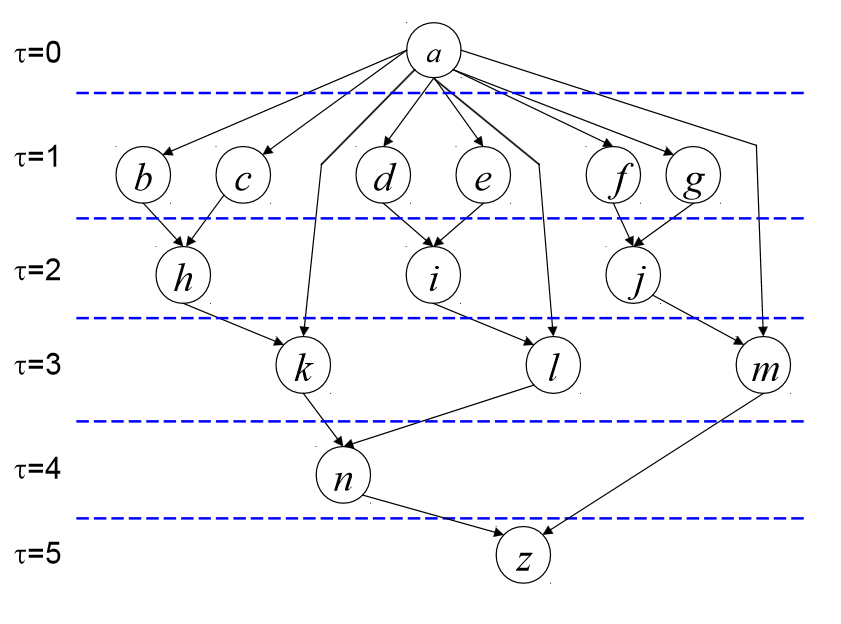
\includegraphics[scale=0.3]{images/asap} \cite{ESDes} \\
	\end{center}
\end{frame}